\chapter{Discussion}

\section{Selecting Working Agreements}


As with any goal, Working Agreements should be achievable. Unrealistic targets tend to be ignored by the team members and can decrease motivation. That said, it is valuable that teams configure Working Agreements left to their own devices. Not all WAs are suitable for all teams: for example, branching strategy needs to be considered during the WA setup.  

Because Working Agreement templates are set by Swarmia, the client teams have limited capacity to select suitable WAs for their needs. Certain presumptions made might make the WAs less valuable or even unusable for some teams: to get the most value out of Swarmia, teams should work with widely accepted CI/CD practices. 

Working Agreements are not intended to be used as primary performance metrics but as a tool that helps teams achieve their objectives. Therefore, it is a safe assumption that teams aim to improve their productivity by enabling WAs. The two most popular WAs, max\_pull\_request\_review\_time and max\_pull\_request\_age, aim to reduce the pull request cycle time. It seems teams using Swarmia are keen on increasing their PR throughput. 

Many practices that WAs introduce are already used in the teams. By using Working Agreements, teams get up-to-date information on their track record and ensure that the rules are followed in the future. 

Most teams enable only a couple of Working Agreements: $64\%$ of teams have configured four or fewer agreements. Teams might test the feature with a couple of agreements and then decide to go all-in if the feature proves helpful. Furthermore, teams usually configure only one Working Agreement per template. A potential reason is related to feature discovery: the possibility of creating multiple agreements might need to be clarified for new teams. The fact that Story is the most popular issue type suggests that most Swarmia teams are acclimated to using Swarmia for Story tracking while Epics, Bugs and Tasks are tracked via other tools like GitHub – or not at all.

\section{Effect of Working Agreements}

\todo[inline]{add more stuff from Swarmia workshop}

Next, we will analyze all independent variables with statistical significance and the potential underlying reasons for the perceived results.

\todo[inline]{Little's law <> wip prs}

wip\_pull\_requests does increase PRCT with a weight of 1.28 and notably high confidence. Especially interesting is that it also increases IPCT. By introducing this working agreement, teams try to limit pull requests on their desk. As the agreement does not directly control the amount of open PRs, it should not form a bottleneck. As the agreement is not forced, the effect on developer behavior is indirect: nothing is stopping them to create more PRs than the set maximum in the WA configuration. 

On the other hand, the PR limit can result in a larger batch size; the amount of changes in a Pull Request increases, which again prolongs review times. While literature suggests that WIP limits are suitable for team productivity~\cite{reinertsen_principles_2009}, in some teams, their overall processes do not support using them. A potential solution would be to intervene earlier, before the limit is exceeded. This could be done with more proactive notifications or even inbuilt limits that disable new PRs before old ones are reviewed and merged. 

no\_direct\_pushes\_to\_main\_branch encourages team members to work through pull requests instead of blindly merging their changes to the main branch. By forcing such a working habit, the teams implement a system where pull requests are approved without a proper review: PRs are made to comply with the working agreement and potential branch protection rules. These for-the-sake-of-it PRs pull down the PRCT: without the WA, PRs probably were made only for the more extensive changes. Even though the rule creates more friction between development and merging to main, reviewing all changes is considered a good practice and should increase code quality. Furthermore, even the rubber-stamped PRs are net-positive for the change history. To get a better touch of this working agreement's potential, we need to use more relevant metrics, such as the change failure rate. 

Pull request review times are considered a common bottleneck in software development \cite{maddila_nudge_2022}. By enabling max\_pull\_request\_review\_time, teams try to encourage themselves to focus on closing open PRs faster. Often review times can prolong due to the inactivity of the author or the reviewer. It is the only WA the personal Slack notifications address: each team member can opt-in to receive direct messages for PRs pending their contribution. The team daily digest also lists open PRs on top, again bringing them to the attention of developers. According to Maddila et al., actively notifying developers of open PRs shortens PR review time.~\cite{maddila_nudge_2022}

\begin{figure}[ht]
    \centering
    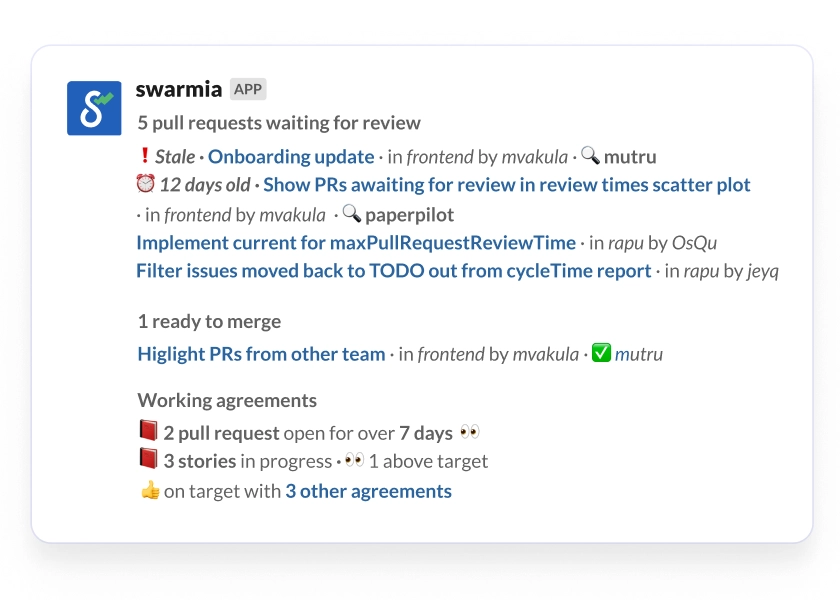
\includegraphics[width=13.5cm]{LaTeX/images/daily-digest.png}
    \caption{Daily Digest, a status report posted by the Slack integration}
    \label{fig:daily_digest}
\end{figure}

The rest of the WAs proved no results that could be trusted due to the lack of statistical significance. Not all Working Agreements aim to reduce cycle times, so naturally, there will not be a direct connection.

\todo[inline]{PRCT does not correlate with issue related WAs. Even though this might seem "logical", one might think that for example wip issues reduces also PR cycle times. add some stuff to discussion 

see results. majority of WAs with impact are PR related! }

\todo[inline]{include SPACE and DORA more}

\section{Studying Teams and Individuals}

\todo[inline]{update to be in line with results. for example, 
slack users and daily digest in IPCT results}

Team members' behavior was observed through three metrics. Even though only slack\_users had statistical significance for cycle times, these metrics can have other influences on team productivity. The number of weekly PR authors, which we assume correlates strongly with team size, did not have a relationship to the cycle times. Although team size and especially the changes in team composition are often considered team performance degrading factors, the results show that team size and cycle times have no connection. 

slack\_users has a weight of $-2.45$ hours per user. For a five-person team, this means that if each team member enables Slack notifications, PRCT decreases by 12 hours. On the other hand, the team-wide notification Daily Digest fails to influence PRCT. Teams integrate the Daily Digest into their current communication channel or create a dedicated channel. As with any high-volume medium, these channels can be flooded with content, causing the notifications to be missed or ignored by the team members.

Meanwhile, the direct message continues to be an efficient way to reach individual contributors. Companies implementing DM notifications should be careful to refrain from spamming developers needlessly. Based on the results, Swarmia has created a valuable personal notification experience. 

\todo{

is it fare to measure metrics the team has not selected as metrics

for example see mail with arto 

}

\section{Directions for Future Work}

In Accelerate, the authors argue that teams should be able to choose their methods and tools~\cite{forsgren_accelerate_2018}. Even though the study only handles monthly active users, it is hard to know their commitment to Swarmia: did they collectively decide to use such a tool and if they did, were the working agreements selected as a team or by a manager?\todo{rewrite without question marks}
 Moreover, the teams' overall motivation for improvement remains to be discovered.

Currently, personal notifications are measured on the top level: whether they are used or not. Variations of the notification could be researched to understand better which notifications have an impact. Future studies could include comparing competing tools, such as GitHub's Slack integration~\cite{noauthor_integrationsslack_nodate}, Microsoft's Nudge Service~\cite{maddila_nudge_2022}, and Swarmia. Furthermore, the length of the effect would need further validation: is the boost achieved by using Slack notifications persistent?\todo{rewrite without question marks}

\todo{add one more potential direction}

\section{Limitations of Work}


\todo{linear model was used even though cycle times > 0 always. which might be not ideal, }

\subsection{Internal validity}

The thesis uses cycle times as a primary metric. Even though reducing cycle times is a goal many teams try to achieve, there are also potential downsides, such as reduced code quality. Frameworks like SPACE and DORA highlight the need for multiple team productivity metrics to find an optimal balance: a single metric cannot reflect all relevant aspects. For example, the change failure rate, which Swarmia already calculates for the customer teams, would bring more depth into the analysis. 

The factors used as independent variables cannot be considered to constitute all the potential factors that may influence PRCT. Factors such as team members' experience or whether teams operate remotely could affect team productivity but were not included in this study. 

Furthermore, the two-year period overlaps significantly with the COVID-19 pandemic, which more or less affected any company. Changes like layoffs, remote work, or pivots cause significant effects on team dynamics. These probable effects must be considered with the available data. On the other hand, Swarmia's client base is highly international and versatile, consisting of companies of all sizes. 

As this is a quantitative study, we rely solely on data available on Swarmia business intelligence tools. Conducting user interviews or surveys would unlock many avenues currently only asserted speculatively. For example, studying perceived performance is more labor-intensive but can shed light on otherwise hard-to-measure dimensions. How people feel they are making progress is a proxy of productivity \cite{forsgren_space_2021}.

\subsection{External validity}

Although we set out to investigate how the Swarmia sub-feature affects team behavior, the aim is to be able to generalize the findings to any other ways of working system. Using Swarmia's Working Agreements is presumably more effective than non-technical implementations, as it actively keeps track of the agreements and nudges team members to stay on track. Therefore, the results achieved in this study are not directly derivative of other team norm systems. 

Furthermore, a tool like Swarmia attracts certain companies more than others. If they are willing to invest in such a tool, they might have more motivation to improve than the companies that decide against using Swarmia or similar tools. 

A positive attribute of the study is that it was conducted using historical data: the teams were unaware that their usage logs would be used as thesis material. 